\documentclass[12pt]{article}
\usepackage[english]{babel}
\usepackage{float}
\usepackage{enumerate, setspace, stackengine}
\usepackage[hidelinks]{hyperref}
\usepackage[margin=1.5cm]{geometry}
\usepackage{geometry}
\geometry{top=1.5cm, left=1.5cm, right=1.5cm, bottom=1.5cm}
\usepackage{caption, subcaption}
\usepackage{amsmath, amsfonts, amssymb}
\usepackage{listings, color}
\usepackage{wrapfig}
\usepackage{graphicx}



\definecolor{dkgreen}{rgb}{0,0.6,0}
\definecolor{gray}{rgb}{0.5,0.5,0.5}
\definecolor{mauve}{rgb}{0.58,0,0.82}

\lstset{frame=tb,
  language=Java,
  aboveskip=3mm,
  belowskip=3mm,
  showstringspaces=false,
  columns=flexible,
  basicstyle={\small\ttfamily},
  numbers=none,
  numberstyle=\tiny\color{gray},
  keywordstyle=\color{blue},
  commentstyle=\color{dkgreen},
  stringstyle=\color{mauve},
  breaklines=true,
  breakatwhitespace=true,
  tabsize=3
}



\title{\textbf{Real Time System}\\ Project\#2}
\author{Team7 - R04922058 Yi Lin Cheng , R04922034 Hsuan-Heng, Wu}
\date{}

\begin{document}
\maketitle

\section*{Part I: Weighted Round Robin Scheduling}
\subsection*{Enqueue task}
	When a new task is created, it needs to be put into \verb|weighted_rr_rq|, which is done by calling \verb|list_add_tail(&H,&E)|.
	This function inserts a new entry E before the specify head H. Thus, given \verb|weighted_rr_rq|'s head as H, E will be inserted at the end of the queue. After inserting E, increase counter \verb|weighted_rr_rq.nr_running| by one.

\subsection*{Dequeue task}
	Deleting a specify task T is done by calling \verb|list_del(&T.list_head)|. This function removes T from the list by modifying \verb|T.list_head|'s pointers and the pointers pointing to \verb|T.list_head|. After removing T, decrease counter \verb|weighted_rr_rq.nr_running| by one.

\subsection*{Pick next task}
	This function is called when OS needs to select the next task to run. Since we want to implement a weighted round robin scheduler, this function should return the first element in \verb|weighted_rr_rq|. We use \verb|list_first_entry()| to retrieve the first element in run queue. Note that we should check if the queue is empty before trying to retrieve an entry. If \verb|nr_running| equals 0, simply return \verb|NULL|.

\subsection*{Task tick}
	Each task has its own time quantum. Every time when \verb|test_tick_weighted_rr()| is called, the quantum of current running task P should be decreased. When a task exhausts its time quantum, the quantum will be replenished but it should yield the CPU and be rescheduled. There are two steps in this function:
	\begin{enumerate}
		\item Decrease P's time quantum:  \verb|p->task_time_slice--|.
		\item If P's quantum is exhausted:\\
			Replenish P's time quantum: \verb|p->task_time_clice=p->weighted_time_slice|.\\
			Move P to the end of the queue: \verb|requeue_task_weighted_rr(rq, P)|.\\
			Specify P needs to be rescheduled: \verb|set_tsk_need_resched(P)|.
	\end{enumerate}

\subsection*{Yield task}
	When a task yields the CPU, it should be moved to the end of run queue. When this function is called, it first retrieves the current running task T by \verb|rq->curr|, then call \verb|requeue_task_weighted_rr(&T)| to move T.

\section*{PART II: Shortest Job First Scheduling}
The implemenation of sched\_sjf.c is mostly based on the implemenation of sched\_weighted\_rr.c. Note that the initial \verb|sjf_time_slice| is assumed to be the execution time of job.
\subsection*{Enqueue task}
	Same as part1.
\subsection*{Dequeue task}
	Same as part1.
\subsection*{Pick next task}
  In shortest job first scheduling implementation, the job with mimimum sjf\_time\_slice should be selected, thus a list\_for\_each call is used to traverse the \verb|sjf->queue| to extract the task with minimum job execution time.
  We use \verb|list_first_entry()| to retrieve the first element in run queue and get its corresponding time\_slice as initial minimum execution time to be later compared throughout iterations.
  Note that we should check if the queue is empty before trying to retrieve an entry. If \verb|nr_running| equals 0, simply return \verb|NULL|.

\subsection*{Task tick}
  The implementation of this function is almost identical to that of part 1. All we need to do is to comment out the section of code where a task is rescheduled if it runs out of time slot because SJF is a no preemption protocol.

\subsection*{Yield task}
  Same as part 1.

\subsection*{Define New Schedule Policy}
  In include\textbackslash linux\textbackslash shed.h , define SCHED\_SJF = 7
\subsection*{Define New System Call}
In arch \textbackslash x86 \textbackslash include \textbackslash asm \textbackslash unistd\_32.h:
  \begin{enumerate}
      \item define \_\_NR\_sched\_sjf\_getquantum 339
      \item define \_\_NR\_sched\_sjf\_setquantum 340
      \item define \_\_NR\_syscalls 343
  \end{enumerate}
In arch \textbackslash x86 \textbackslash kernel\textbackslash syscall\_table\_32.S
  \begin{enumerate}
    \item append .long sys\_sched\_sjf\_getquantum
  	\item append .long sys\_sched\_sjf\_setquantum
  \end{enumerate}
In include \textbackslash linux \textbackslash syscalls.h
  \begin{enumerate}
    \item append asmlinkage long sys\_sched\_sjf\_getquantum(void);
    \item append asmlinkage long sys\_sched\_sjf\_setquantum(unsigned int quantum);
  \end{enumerate}
\subsection*{Update Sched.c}
  include sched\_sjf.c
  In kernel\textbackslash sched\_.c
  \begin{enumerate}
    \item add sjf\_rq
    \item define and implement sched\_sjf\_getquantum
    \item define and implement sched\_sjf\_getquantum
    \item define sjf\_time\_slice
  \end{enumerate}

\subsection*{Concatenate list of sched\_classes}
  In kernel\textbackslash sched\_weighted\_rr.c
  \begin{enumerate}
    \item update weighted\_rr\_sched\_class.next = sjf\_sched\_class
  \end{enumerate}
  In kernel\textbackslash sched\_sjf.c
  \begin{enumerate}
    \item update sjf\_sched\_class.next = idle\_sched\_class
  \end{enumerate}

  \section*{Part III: Rate Monotonic Scheduling}
  The implementation of Part 3 is based on recompiliing the kernel with different version of sched\_sjf.c using SCHED\_SJF due to some unknown error that prevents SCHED\_RMS to work. Thus , for sched\_rms.c to work, it must be renamed to sched\_sjf.c and replace the original one such that sched\_sjf.c will perform different policies.

  \subsection*{Enqueue task}
  	Same as part 1.
  \subsection*{Dequeue task}
  	Same as part 1.
  \subsection*{Pick next task}
  	Same as part 2 , since we assign task we lower period higher priority.

  \subsection*{Task tick}
  	Similar to part 1, but since Rate Monotonic allows preemption, we need to check whether there are tasks with higher priority in the task\_queue. This is done by a list\_for\_each iterative check and an additional or check for rescheduling.

  \subsection*{Yield task}
  	Same as part 1.

\section*{Part IV: Test Cases}
  \subsection*{For Part II}
    In the for loop that creates pthread, add random time quantum to the base time quantum , and set the last thread created to the highest possible priority ( lowest execTime). The design of last thread with lowest execTime is used to test whether preemption is successfully disabled.
  \subsection*{For Part III}
    Similar to the case for part II, except that a usleep call is performed before the creation of last thread, this design is used to test whether preemption can happen at every tick.

\section*{Result}

	\begin{figure}[H]
	\centering
	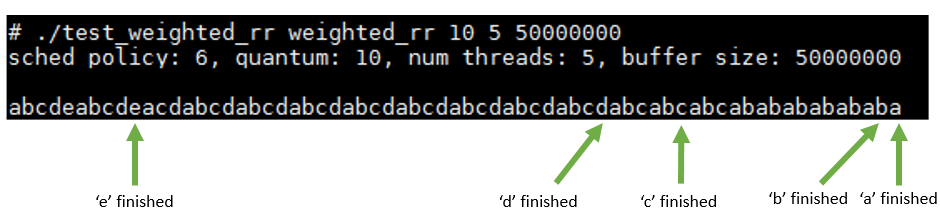
\includegraphics[width=1\textwidth]{fig_result_1}
	\caption{Result of Part I} \label{fig:result1}
	\end{figure}

  \begin{figure}[H]
	\centering
	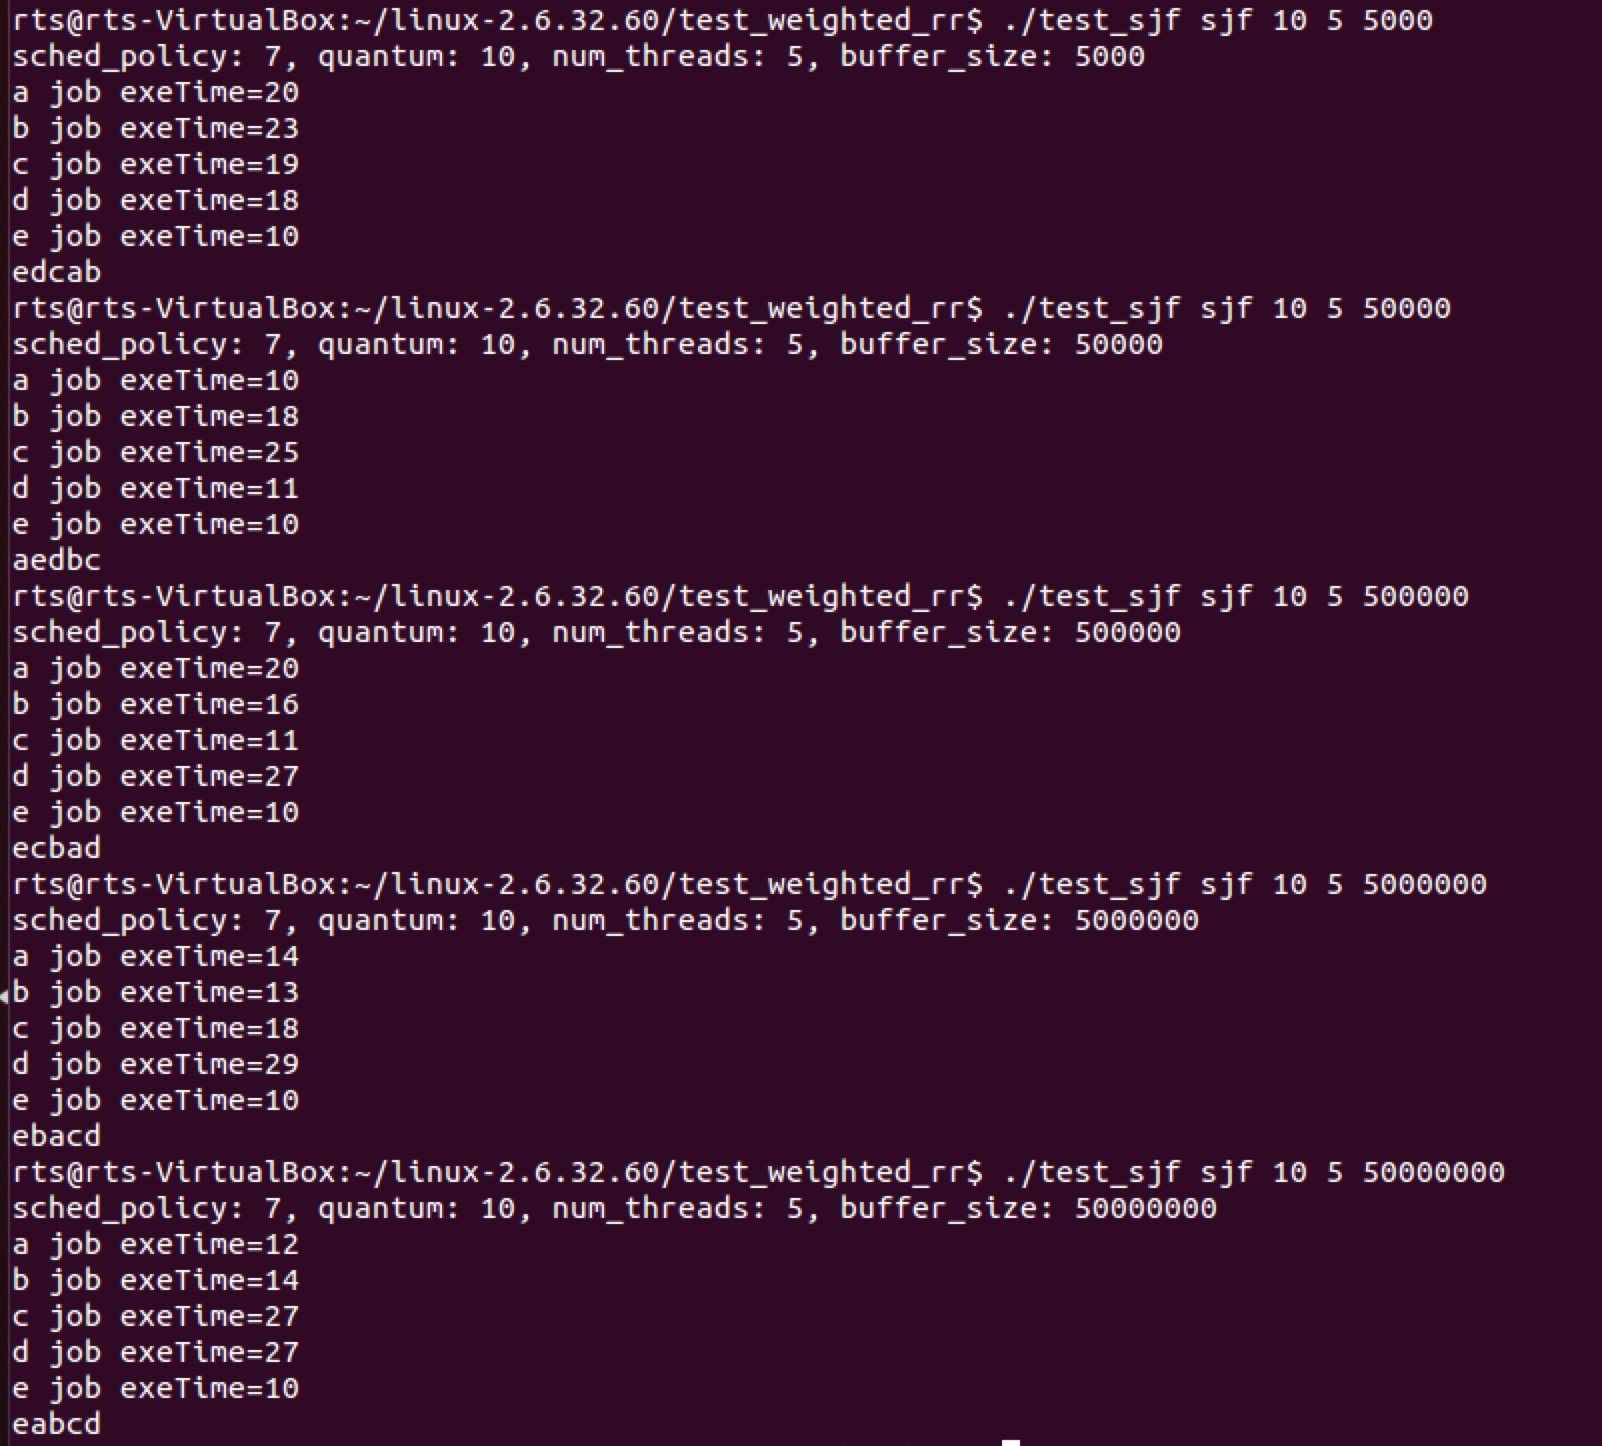
\includegraphics[width=1\textwidth]{fig_result_2}
	\caption{Result of Part II} \label{fig:result2}
	\end{figure}

  \begin{figure}[H]
	\centering
	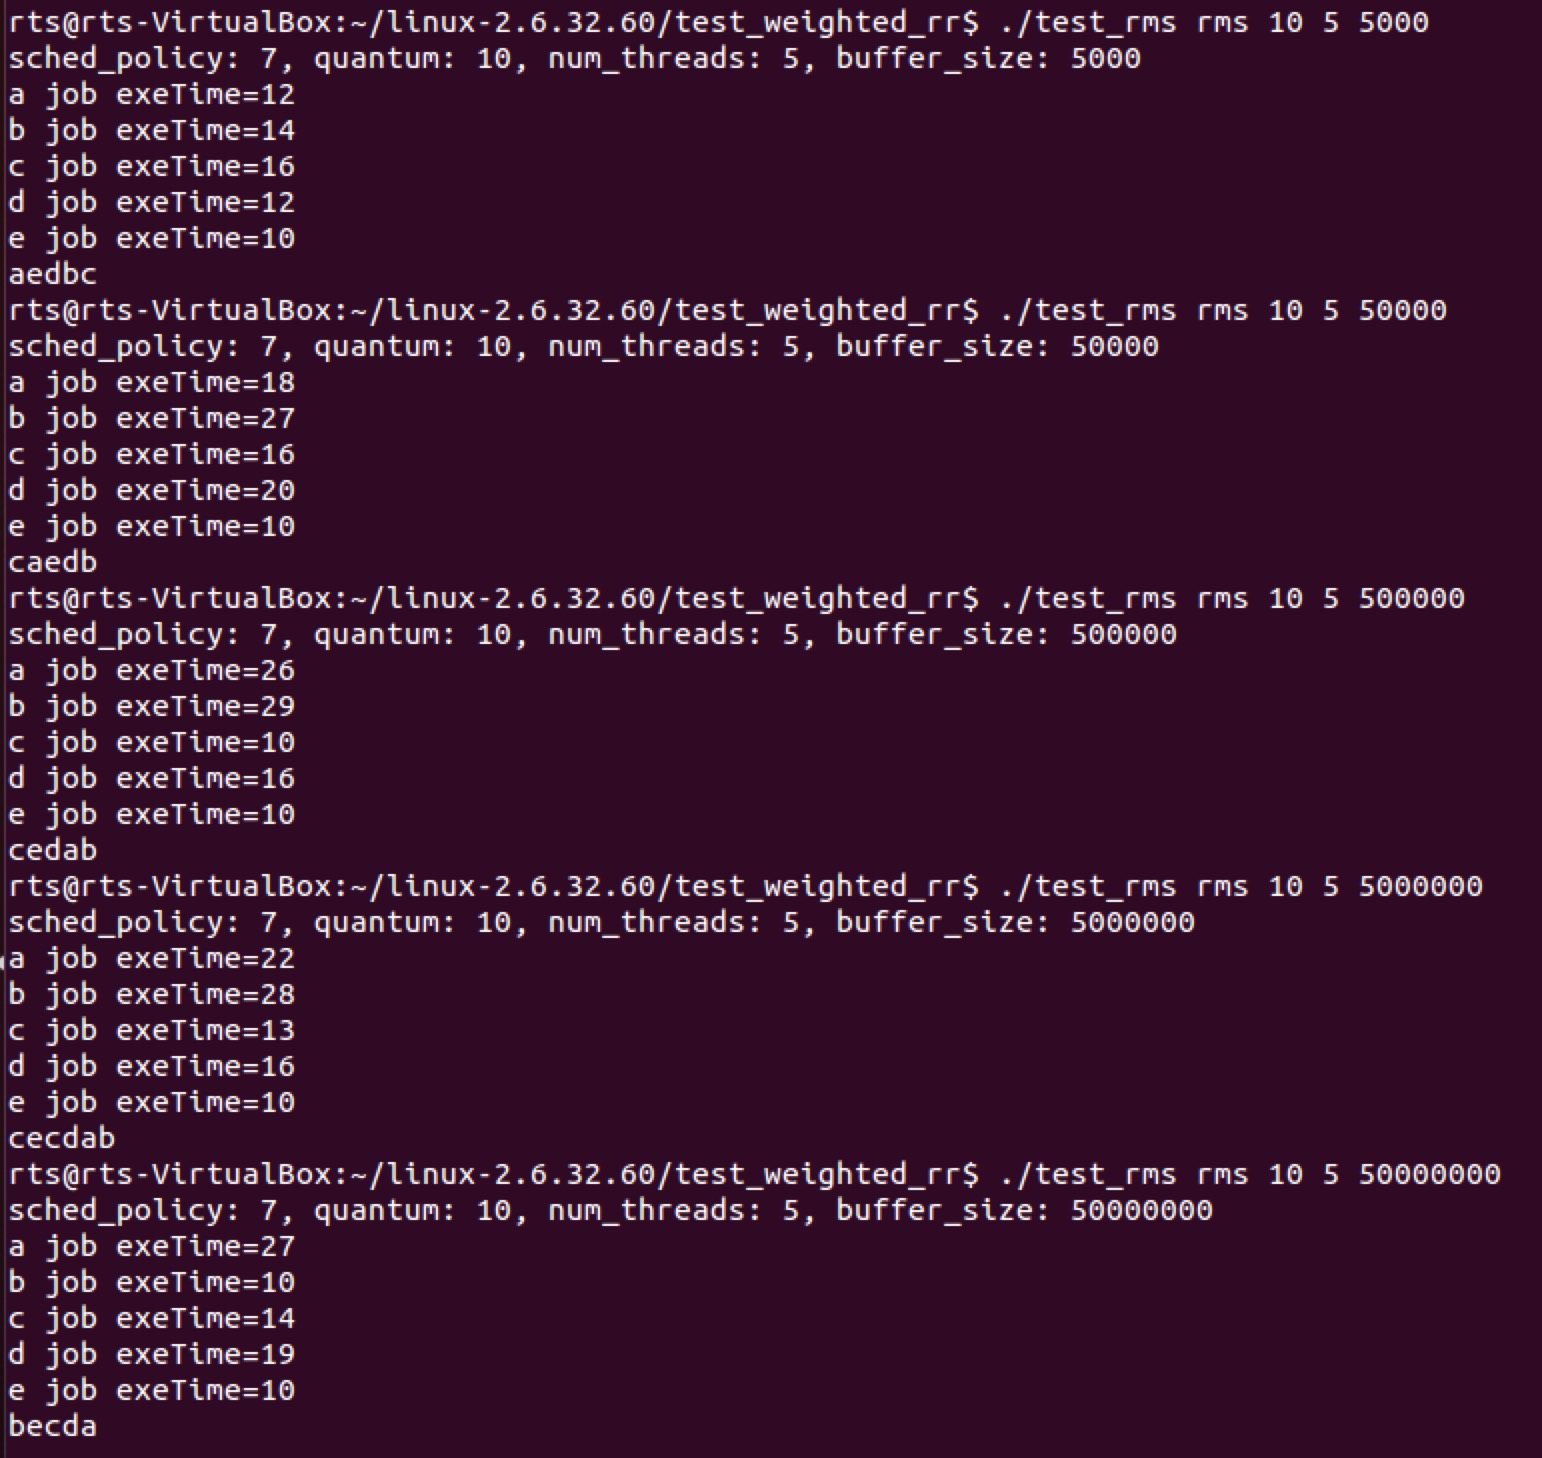
\includegraphics[width=1\textwidth]{fig_result_3}
	\caption{Result of Part III} \label{fig:result3}
	\end{figure}
\end{document}
